\section{有限和与期望目标}
\label{sec:opt-sto-objectives}

随机算法里有两种随机性容易混在一起：数据本身是从某个总体中抽来的，算法每一步又随机挑选读取哪些数据。前者决定我们在优化哪个函数，后者只决定求解过程看到哪些信息。本节先把被优化的目标固定下来，说明一次完整梯度要付出什么代价，再把有限平均推广到期望，并指出微分与期望交换所需的条件。后面各节的分析都针对这里选定的目标。

\subsection{固定样本的有限和}
\label{sec:opt-sto-finite-sum}

\paragraph{逐项平均的目标}
机器学习中的目标通常是逐样本损失的平均。给定$n$个样本，第$i$个样本贡献一个函数$f_i:\mathbb R^d\to\mathbb R$，目标是
\begin{equation}
\label{eq:opt-sto-finite-sum}
  f(\bm x)=\frac1n\sum_{i=1}^n f_i(\bm x).
\end{equation}
这种形式称为\term{有限和目标}（finite-sum objective）。正则项可以平均分摊到每一项里，也可以单独写出。本章的主要例子是岭回归形式的最小二乘：取$\bm A\in\mathbb R^{n\times d}$的第$i$行为$\bm a_i^\top$，
\[
  f_i(\bm x)=\tfrac12(\bm a_i^\top\bm x-b_i)^2+\tfrac{\lambda}{2}\lVert\bm x\rVert_2^2,\qquad
  f(\bm x)=\frac1{2n}\lVert\bm A\bm x-\bm b\rVert_2^2+\frac{\lambda}{2}\lVert\bm x\rVert_2^2 .
\]
它与本部分通用的写法$\tfrac12\lVert\bm A\bm x-\bm b\rVert_2^2+\tfrac{\lambda'}{2}\lVert\bm x\rVert_2^2$只差整体因子$1/n$和记号$\lambda'=n\lambda$，最小点相同。这里除以$n$，是为了让目标值和梯度的量级不随样本数增长，步长也就不必随$n$重新换算。

\paragraph{一次完整梯度的代价}
完整梯度$\nabla f(\bm x)=\frac1n\sum_i\nabla f_i(\bm x)$需要读取全部$n$项。对上面的最小二乘，$\nabla f_i(\bm x)=\bm a_i(\bm a_i^\top\bm x-b_i)+\lambda\bm x$，一项的计算量是$O(d)$，完整梯度是$O(nd)$。$n$达到百万、数据存放在磁盘或分布在多台机器上时，读一遍数据本身就是主要开销。相比之下，只读一项的代价与$n$无关。本章所说的“少读取”，指的就是用一部分项的梯度代替这$n$项的平均。

需要强调的是，数据一旦固定，$f$就是一个确定的函数，它的最小点、最优值和梯度都没有随机性。随机抽取下标只改变算法在某一步获得的信息：同一个点$\bm x$，抽到不同的项会读到不同的向量。后面说“随机梯度的期望等于梯度”，期望是对抽样下标取的，被比较的仍是这个确定目标的梯度。

\begin{example}[三点平均]
\label{ex:opt-sto-three-points}
取$d=1$、$n=3$，$f_i(x)=\tfrac12(x-c_i)^2$，$c_1=0$、$c_2=1$、$c_3=5$。目标
\[
  f(x)=\frac16\bigl(x^2+(x-1)^2+(x-5)^2\bigr)=\frac12(x-2)^2+\frac73
\]
在$x^\star=2$处取得最小值$f^\star=7/3$，它是$1$强凸、$1$光滑的。在$x=3$处，三项的梯度$x-c_i$分别是$3$、$2$、$-2$，平均为$1=f'(3)$。第三项的读数$-2$与真梯度符号相反：如果这一步只看它，就会向右走，离最小点更远。这个例子会在本章反复使用，因为每项曲率相同，许多量可以精确算出。
\end{example}

\paragraph{目标项分解与变量分块}
减少计算还有另一个方向。有限和把目标按\emph{项}拆开，读取其中一部分；变量分块则把$\bm x$按\emph{坐标}拆成若干块，每轮只更新其中一块，其余坐标保持不变。图~\ref{fig:opt-sto-sum-vs-block}把两者画在同一个数据矩阵上：前者选行，后者选列。两者互不排斥，例如可以抽一批样本、只更新这批样本涉及的那些坐标。但每种节省都改变了“一步”的含义，因此分析时必须记录每次调用的三样东西：在哪个点求值，按什么分布抽取了哪些项或哪些坐标，返回了什么向量。后文的收敛结论都依赖于这些记录满足的条件。

\begin{figure}[!htbp]
  \centering
  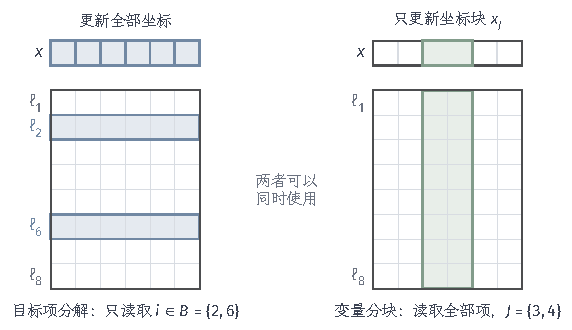
\includegraphics[width=96.855mm]{figures/03-optimization-evolution-and-signals/01-optimization/tikz/c6-sum-vs-block/figure.pdf}
  \caption{同一个数据矩阵上的两种节省。网格的$8$行对应$8$个目标项$\ell_i$，$6$列对应决策变量的$6$个坐标，顶部一行表示$\bm x$。左：目标项分解，本轮只读取第$2$、$6$行（蓝色），但所得方向更新全部坐标。右：变量分块，本轮读取全部行，只更新第$3$、$4$个坐标组成的块$\bm x_J$（绿色）。}
  \label{fig:opt-sto-sum-vs-block}
\end{figure}

\subsection{期望目标与随机梯度}
\label{sec:opt-sto-expectation}

\paragraph{从有限平均到期望}
有限和是一种特殊的期望：令下标$I$在$\{1,\dots,n\}$上均匀分布，就有$f(\bm x)=\mathbb E[f_I(\bm x)]$。更一般地，设$\xi$是取值于某个空间的随机变量，$f(\bm x;\xi)$是给定$\xi$时的损失，目标
\begin{equation}
\label{eq:opt-sto-expectation}
  F(\bm x)=\mathbb E_\xi\bigl[f(\bm x;\xi)\bigr]
\end{equation}
称为期望目标。按照能否获得$\xi$的分布，可以分三种情形。若分布已知且期望能算出闭式，$F$就是普通的确定目标。若只能从分布中采样，例如数据持续到来、每个样本只用一次，那么每次采样得到一个新的读数，算法直接面对$F$。若先收集$n$个样本$\xi_1,\dots,\xi_n$，再用$\frac1n\sum_if(\bm x;\xi_i)$代替$F$，就回到有限和~\eqref{eq:opt-sto-finite-sum}，这个平均在学习问题中称为\term{经验风险}（empirical risk），$F$则对应\term{期望风险}（expected risk）。

\paragraph{微分与期望何时可交换}
期望目标的随机梯度通常取为$\nabla_{\bm x}f(\bm x;\xi)$。要让它的期望等于$\nabla F(\bm x)$，需要把梯度移到期望里面。积分号下求导定理给出一个常用的充分条件：若在$\bm x$的某个邻域内，对几乎每个$\xi$，$f(\cdot;\xi)$可微，且偏导数被一个可积函数$G(\xi)$统一控制，$\lVert\nabla_{\bm x}f(\bm y;\xi)\rVert_2\leq G(\xi)$对邻域内所有$\bm y$成立，$\mathbb E[G(\xi)]<\infty$，同时$f(\bm x;\cdot)$本身可积，则$F$在$\bm x$可微且$\nabla F(\bm x)=\mathbb E[\nabla_{\bm x}f(\bm x;\xi)]$。该定理的证明基于中值定理与控制收敛定理，可参考\BookChapterRef{chap:integration}{卷二“积分”章}；这里只用它的结论。有限和情形下期望是有限加权和，只要每项可微，交换自动成立。

条件不满足时，交换可能失败，而且失败的方式很隐蔽。设$\xi$在$[0,1]$上均匀分布，$f(x;\xi)=\mathbb 1_{\{\xi\leq x\}}$。对$x\in(0,1)$，$F(x)=\mathbb P(\xi\leq x)=x$，导数为$1$。可是对每个固定的$\xi\neq x$，$f(\cdot;\xi)$在$x$附近是常数，逐样本导数为零，于是$\mathbb E[\partial_xf(x;\xi)]=0\neq1$。问题出在跳跃点$\xi$随样本移动：差商$(f(x+h;\xi)-f(x;\xi))/h$在一个概率为$h$的集合上等于$1/h$，无法被与$h$无关的可积函数控制。目标在平均意义下光滑，不代表逐样本的梯度可以拿来作无偏读数。第~\ref{sec:opt-sto-surrogate}节的离散前向会再遇到这种现象。

\paragraph{估计总体梯度与求解经验目标}
在学习问题里，人们最终关心的常是期望风险$F$，手里却只有固定的$n$个样本。这时存在两种不同的误差。其一来自数据：经验风险的最小点与期望风险的最小点不同，这个差距由样本量和模型决定，再精确地求解经验风险也消除不了。其二来自计算：在固定的经验风险上，算法跑了有限步，返回点与经验最小点之间还有差距。本章研究的是后一种：选定一个目标（有限和或期望），分析算法在有限步后能把这个目标的误差降到多少。经验最小点与总体最小点之间的差距、模型选择与泛化保证属于统计问题，由后续讨论学习理论的部分承担。两种误差可以相互权衡，例如数据有限时不必把优化误差压到远低于统计误差的水平，但它们的来源与控制手段不同，不能用同一个数字代表。
